\chapter{Instrument analysis for a cold source}
\label{chapter:introduction}
\label{c3}
\begin{figure}[hbtp]
	\centering
	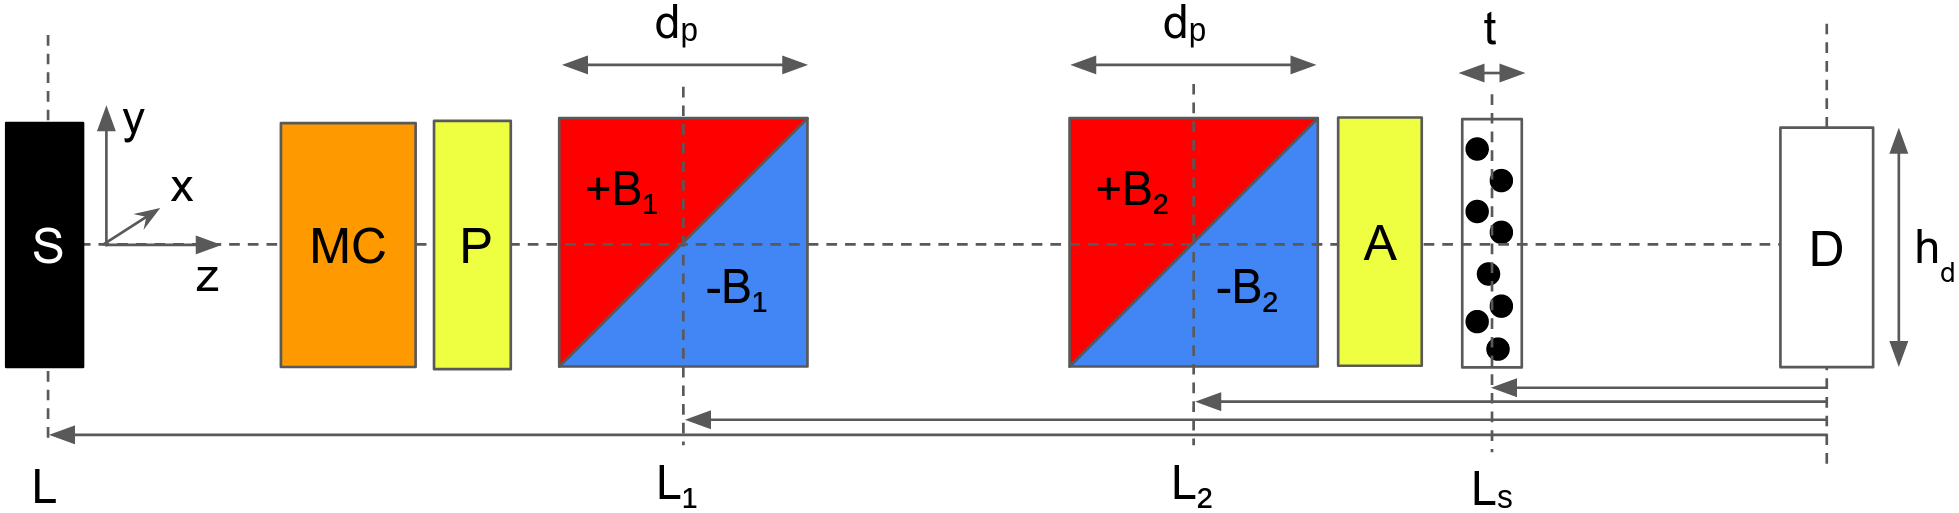
\includegraphics[width=\linewidth]{instrument-configuration}
	\caption{A schematic of the SEMSANS instrument configuration considered in this chapter. Lengths and dimensions are not to scale. Neutrons are emitted from the source (S) after which they pass through a monochromator (MC) and are polarized in the $+x$ direction by a polarizer (P). The polarized neutrons travel through two precession devices (shown are Wollaston prisms as discussed in Section \ref{c3.3}) at distances $L_1, L_2$ from the detector. These devices have field strength $\pm B_1$ and $\pm B_2$ in different field regions to create a $y$-dependence in the precession angle as discussed in Section \ref{c2.2} and have depth $d_p$. Next, the beam passes through an analyzer (A) which can be in the $+x$ or $-x$ setting, creating a modulated intensity pattern. This modulated beam scatters of the sample with thickness $t$ at distance $L_s$ from the detector, arriving at the detector (D) with height $h_d$. The sample can be removed to measure the unscattered modulation pattern, making it possible to compute the decrease in modulation visibility related to $G(\delta)$ as per Equation \eqref{eq:sample-pol-reduction}.}
	\label{fig:instrument-config}
\end{figure}

In this chapter, the used SEMSANS instrument model is introduced and analysed. The cold neutron source and the applicable monochromators for different $\lambda_0$ ranges will be described and three different precession device options and their properties will be discussed. Additionally, the effect of a spread in wavelength $\lambda$ on the observed modulation pattern as well as what is effectively measured will be considered. This is to account for the greater wavelength spread $\Delta\lambda/\lambda_0$ encountered when using a velocity selector as monochromator, which is necessary at higher $\lambda_0$ operating points accessible at a cold source. In the last section, a list of instrument design variants considered in this research is introduced. These will be analysed and simulated in Chapter \ref{c4:constraints} and Chapter \ref{c6:monte-carlo} respectively. 

\section{Instrument configuration}
\label{c3.1}
The general SEMSANS instrument model considered in this work is illustrated in Figure \ref{fig:instrument-config}. It is derivative of an existing study simulating a SEMSANS instrument using ferromagnetic foil-flippers and the corresponding McStas instrument \texttt{SEMSANS\_Delft} \cite{bouwman2021b}. Neutrons enter the instrument from a source, after which they pass through a monochromator set to select neutrons with a wavelength around $\lambda_0$, with  $\Delta\lambda/\lambda_0$ depending on the choice of monochromator as described below. Next, they pass through a polarizer and two precession devices at locations $L_1, L_2$ respectively. As described in Chapter \ref{c2:theory}, a modulated neutron intensity pattern appears after the analyser, which scatters of the sample at distance $L_s$ from the position-sensitive detector at the end, causing different degrees of loss of visibility of the modulation pattern depending on the sample structure as discussed in Section \ref{c2.3}. 

\section{Source beam characteristics and monochromators}
\label{c3.2}
The cold source is assumed to have a spectrum corresponding to a Maxwell-Boltzmann distribution at $T = \SI{20}{\kelvin}$ given by 
\begin{equation}
	f_\lambda(\lambda) = \sqrt{\frac{2}{\pi}}\left(\frac{1}{mk_BT}\right)^{\frac{3}{2}}\frac{h^3}{\lambda^4}e^{-\frac{h^2}{2k_BTm\lambda^2}} \label{eq:cold-source-spectrum}
\end{equation}
This distribution is shown in Figure \ref{fig:source-spectrum}, with the thermal distribution at $T= \SI{290}{\kelvin}$ also shown for reference. For simplicity, a uniform rectangular beam of size $10\times10~\unit{\milli\meter}$ is used to model the beam and it is focussed on the middle $10\times10~\unit{\milli\meter}$ of the detector. Each neutron originating from point $(b_x,b_y)$ in the beam will be aimed at a uniformly sampled random point $(d_x, d_y)$ on the detector, so assuming a distance $L = \SI{5}{\meter}$ from source to detector the divergence will be at most $\psi_0 = \SI{2}{\milli\radian}$ along the $x$ or $y$ axis and about $\psi_0 = \SI{2.8}{\milli\radian}$ in total. This model corresponds to a rectangular setting of the \texttt{Source\_simple} McStas source component which will be used in Monte Carlo simulations in Chapter \ref{c6:monte-carlo}.  

% The peak for $T= \SI{20}{\kelvin}$ corresponds to $E = k_bT = \SI{1.7}{\milli\electronvolt}$ as opposed to $E = \SI{25.0}{\milli\electronvolt}$ for thermal neutrons. 
\subsection{Monochromators}
A monochromator is used to select a narrow band of wavelengths around a central wavelength $\lambda_0$. In a practical instrument, a pyroletic graphite (PG) crystal monochromator can be used to do this up to roughly $\lambda_0 \approx \SI{4.4}{\angstrom}$. For greater wavelengths, a velocity selector (VS) can be used to select neutrons travelling at the right velocity. This is a mechanical device rotating at a great speed, and a lower practical limit of $\lambda_0 \approx \SI{7}{\angstrom}$ is used as lower $\lambda_0$ would require a too great RPM. Both types of monochromator are characterized by $\Delta\lambda/\lambda_0$, the ratio of the full-width-half-maximum (FWHM) of wavelengths $\Delta\lambda$ passed through and $\lambda_0$. In PG crystals, this is a function of the mosaicity of the crystal \cite{shapiro1972} and for velocity selectors it depends on the ratio of the angular aperture of slits and the pitch angle \cite{szewc2010}. This ratio is taken to be $\Delta\lambda/\lambda_0 = 0.01$ and $\Delta\lambda/\lambda_0 = 0.1$ for the PG monochromator and velocity selector respectively, roughly corresponding to the characteristics of components available for an eventual realization. The transfer of these monochromators is taken to be a Gaussian centered at $\lambda_0$ with $\sigma = \frac{1}{2\sqrt{2\ln 2}}\Delta\lambda$, resulting in a selected $\lambda$-spectrum that can be approximated as Gaussian. This motivates the use of the following Gaussian distribution as spectrum after the monochromator in both analysis and simulations.
\begin{equation}
	f_\text{gauss}(\lambda) = \frac{1}{\sigma\sqrt{2\pi}} e^{-\frac{1}{2}(\frac{\lambda - \lambda_0}{\sigma})^2} \label{eq:gauss-spectrum}
\end{equation}
\begin{figure}
	\centering
	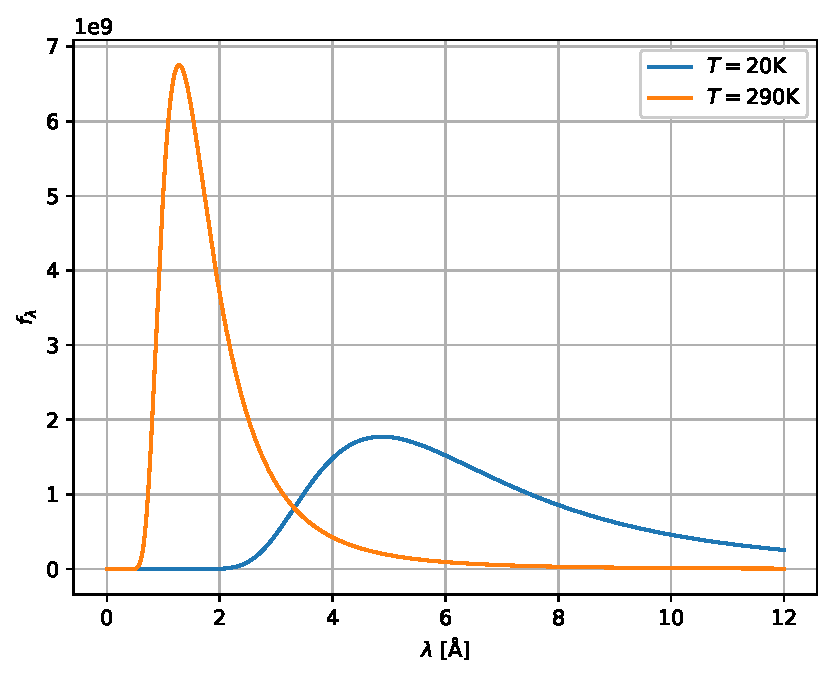
\includegraphics[width=0.5\linewidth]{source-spectrum}
	\caption{Probability density function for Maxwell-Boltzmann neutron sources at $T = \SI{20}{\kelvin}$ and $T = \SI{290}{\kelvin}$, illustrating the spectral differences. }
	\label{fig:source-spectrum}
\end{figure}
%% TODO: Discuss collimation, how the source in simulations will be focussed on the detector in a certain way etc. This lends itself to the language of collimation, divergence etc.
\section{Precession device analysis}
\label{c3.3}
As discussed in Chapter \ref{c2:theory}, different precession devices can be derived that give a precession angle of the form of Equation \eqref{eq:precession-freq} resulting in modulation. The three main types existent in literature are isosceles triangles \cite{sales2015}, magnetic Wollaston prisms \cite{li2021} and ferromagnetic foil flippers \cite{bouwman2021b} and all three have previously been used in SEMSANS realizations and simulations. Their respective geometries are shown in Figure \ref{fig:precession-devices}. What they all have in common is that their effect is proportional to $\cot(\theta_0)$ and magnetic field strength $B$. Here, $\theta_0$ is the angle the magnetic field interfaces make with the $z$-axis in the $yz$ plane.
\subsection{Isosceles triangles}
In the case of a triangle as illustrated in Figure \ref{fig:precession-devices:iso}, the angle of the faces with the $z$-axis can be seen to be $\theta_0 = \arctan\left(\frac{h}{d/2}\right)$. Consider the triangle to be centred along the optical axis so that $y=0$ bisects it. Then for a path at height $y$, the length $L$ passed through the field becomes
$$L = d/2 - \frac{2y}{\tan\theta_0}$$
Using the Equation \eqref{eq:larmor-prec}, the precession angle after passing through the triangle becomes
$$\phi = c\lambda B L = c\lambda B(d/2 - \frac{2y}{\tan\theta_0})$$
Next, consider two similar triangles with base $d_1, d_2$ and field strengths $B_1, B_2$. Adding their precession angles gives 
$$\phi = c\lambda (B_1d_1/2 +B_2d_2/2) - 2c\lambda (B_1 + B_2) \frac{y}{\tan\theta_0}$$
To achieve $\phi = 0$ at $y=0$, the condition $B_1d_1 = -B_2d_2$ must hold, giving 
$$\phi = -2c\lambda (B_1 + B_2) \frac{y}{\tan\theta_0}$$
This can be achieved by making the triangle with the stronger field the smallest. 

\subsection{Magnetic Wollaston prisms}
A more sophisticated device is the magnetic Wollaston prism shown in Figure \ref{fig:precession-devices:wsp}, having two equal and opposite triangular magnetic fields in the form of a square. The analysis is very similar to that of isosceles triangles and for a single prism with angle $\theta_0$, the precession angle is
$$\phi = \frac{2c\lambda B y}{\tan{\theta_0}}$$
Two prisms with fields $B_1, B_2$ in sequence gives
$$\phi = \frac{2c\lambda (B_1 + B_2) y}{\tan{\theta_0}}$$
\subsection{Ferromagnetic foil flippers}
The last device type considered is the ferromagnetic foil flipper depicted in Figure \ref{fig:precession-devices:foil}. It consists of a ferromagnetic foil of thickness $d = \SI{3}{\micro\meter}$ in an electromagnet which quickly saturates to a magnetization of $B_s = \SI{1.0}{\tesla}$ \cite{kraan2003}. The foil has the effect of rotating neutron spins around it by an angle 
$$\phi_{foil} = \frac{cdB_s\lambda}{\sin\theta_0}$$
By appropriately choosing $\theta_0$, the foil can be made to rotate a central wavelength $\lambda_0$ by $\phi_{foil} = \pi$, causing the device to emulate a magnetic Wollaston prism using a simpler magnetic field as the effect of the second triangular region behind the foil will be opposite to that of the first for $\lambda = \lambda_0$. In this case,
$$\phi = -2c\lambda (B_1 + B_2) \frac{y}{\tan\theta_0}$$
For $\lambda \neq \lambda_0$ this will cause a depolarization as was previously shown experimentally \cite{kraan2003}.
% I think because there is then a y-component of spin which shows up as 50/50 up/down on the detector. 
\begin{figure}[htbp]
	\centering
	\begin{subfigure}[b]{0.3\textwidth}
		\centering
		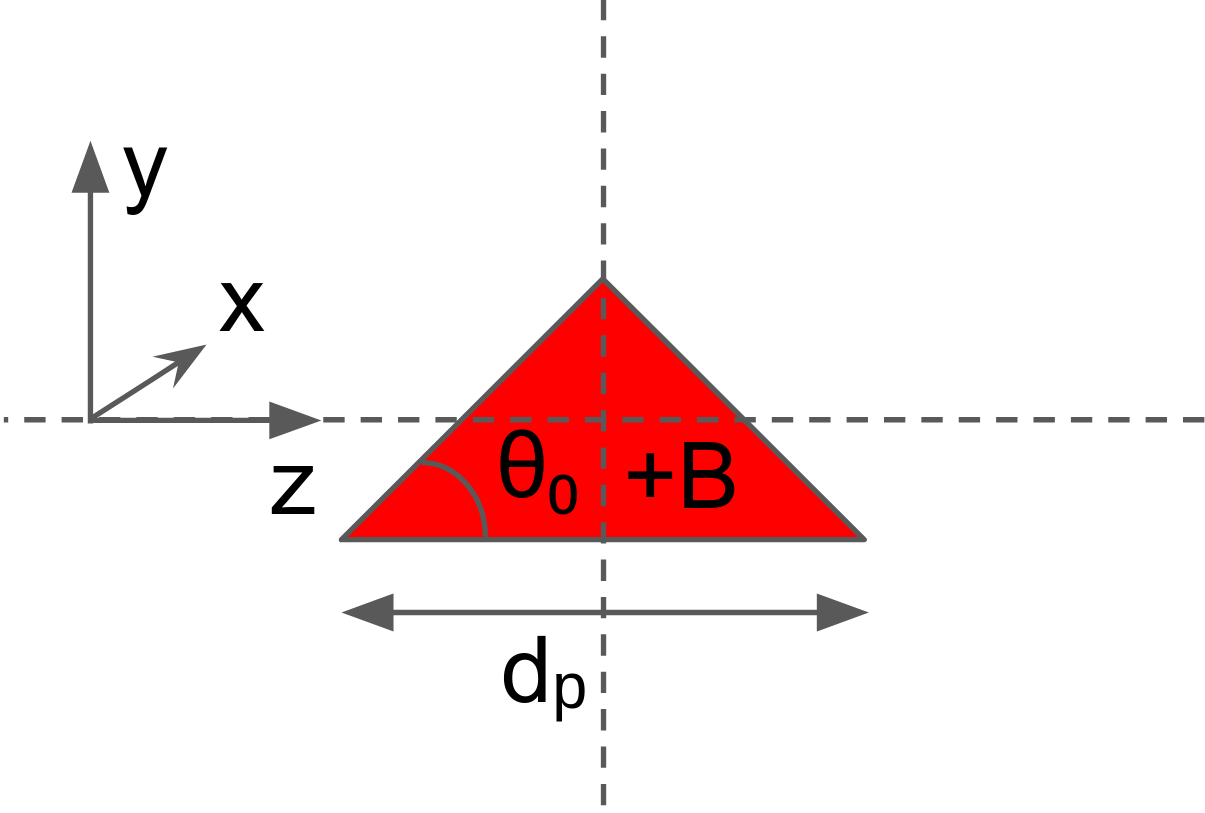
\includegraphics[width=\textwidth]{iso-schematic}
		\caption{Isosceles triangle}
		\label{fig:precession-devices:iso}
	\end{subfigure}
	\hfill
	\begin{subfigure}[b]{0.3\textwidth}
		\centering
		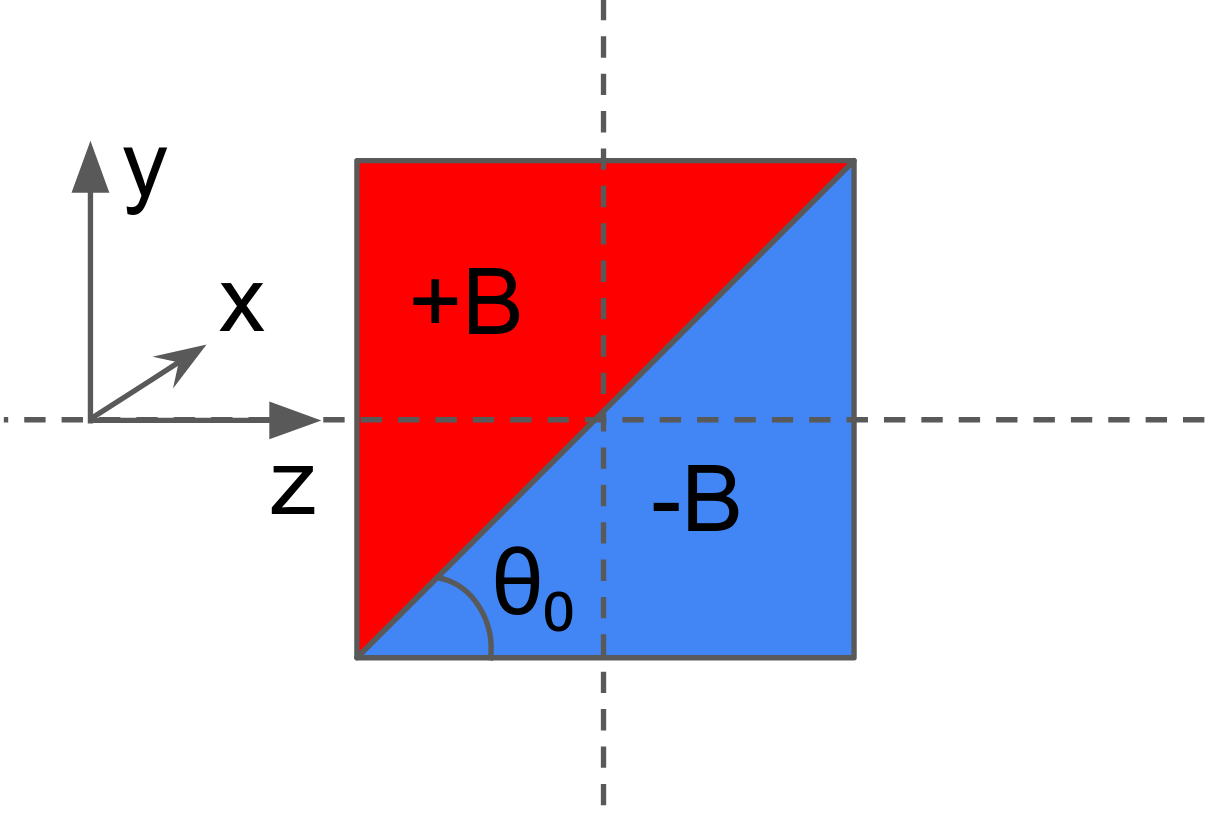
\includegraphics[width=\textwidth]{wp-schematic}
		\caption{Magnetic Wollaston prism}
		\label{fig:precession-devices:wsp}
	\end{subfigure}
	\hfill
	\begin{subfigure}[b]{0.3\textwidth}
		\centering
		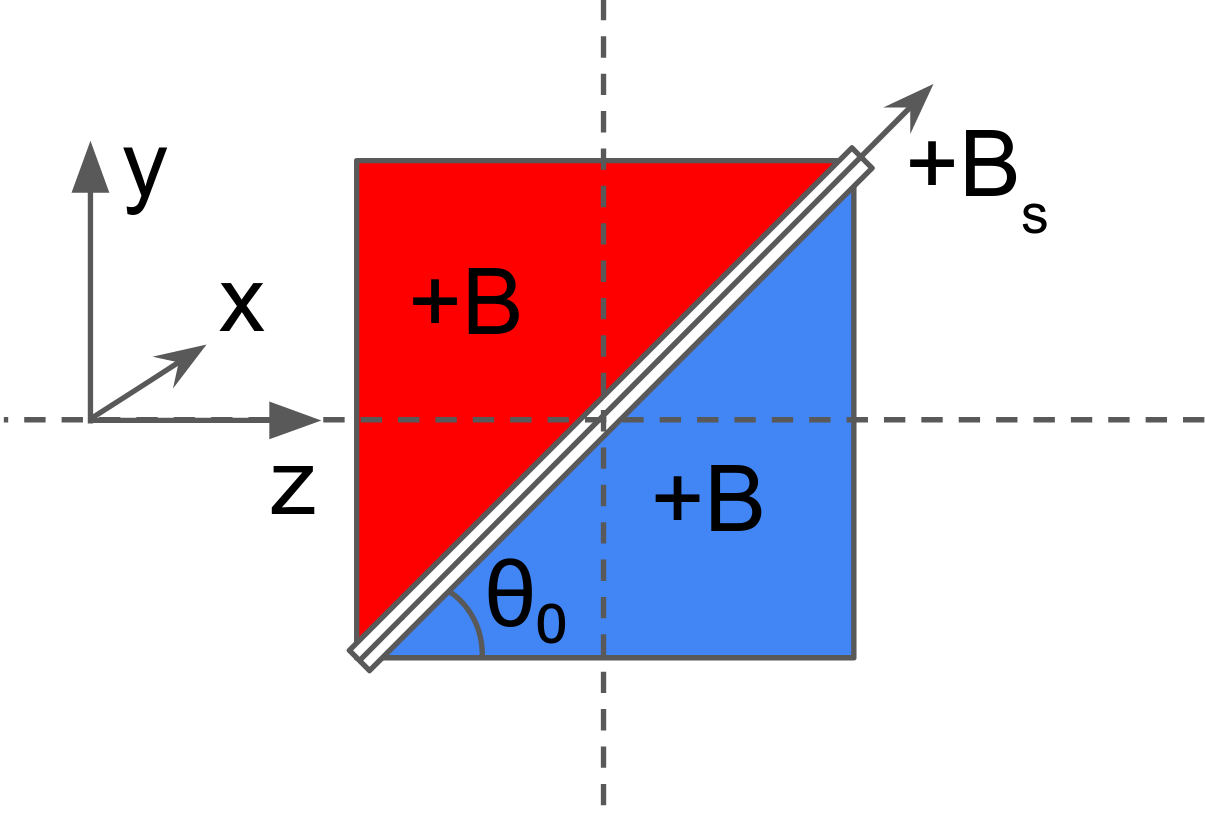
\includegraphics[width=\textwidth]{foil-schematic}
		\caption{Ferromagnetic foil flipper}
		\label{fig:precession-devices:foil}
	\end{subfigure}
	\caption{Schematics for the three different types of precession devices. Assuming positive $B$, the red areas represent a magnetic field in the $+y$ direction and blue areas a field in the $-y$ direction, with exception of Figure \ref{fig:precession-devices:foil}. The reason for this is that the strong $B_s$ field inside the ferromagnetic foil effectively flips the precession of neutrons of the right $\lambda_0$, causing the positive field after the foil to have the effect of a negative field, simulating the fields seen in a Wollaston prism as shown in Figure \ref{fig:precession-devices:wsp}. For all precession devices the field interfaces are canted by $\theta_0$ in the $yz$-plane and all have depth $d_p = \SI{0.3}{\meter}$ as indicated in Subsection \ref{c3.3.4}. Only for Wollaston prisms $\theta_0 = \SI{45}{\deg}$ as shown, with isosceles triangles in practice having $\theta_0 = \SI{20}{\deg}$ and $\theta_0$ being a function of $\lambda_0$ in the case of foil flippers.}
	\label{fig:precession-devices}
\end{figure}

\subsection{Device $\alpha$ and characteristics}
\label{c3.3.4}
To summarize the above discussion of the three available devices, once device-specific conditions are met a pair of any of them have in absolute terms the same precession-angle profile given by Equation \eqref{eq:precession-freq} with $\alpha = \frac{(B_1 + B_2)}{\pi\tan\theta_0}$
\begin{equation}
	\phi = 2c\lambda (B_1 + B_2)\frac{y}{\tan\theta_0} \label{eq:device-prec}
\end{equation}
the contribution of each separate device being $\phi_i = \frac{2c\lambda B_i y}{\tan\theta_0}$. $\theta_0$ is a function of $\lambda_0$ for foil flippers and is fixed for Wollaston prisms and isosceles triangles, meaning that $B_1, B_2$ will in practice be set to vary $\alpha$. Table \ref{tab:device-properties} summarizes device characteristics as they appear in literature that will be used in this research. All devices are assumed to have depth $d_p = \SI{0.3}{\meter}$, limiting possible values of $L_1, L_2$ and $L_s$. 
\begin{table}[h!]
	\centering
	\begin{tabular}{c|c c c c c}
		\toprule
		Name & Label & $\theta_0~[\unit{\degree}]$ & $B_{\text{min}}~[\unit{\milli\tesla}]$ & $B_{\text{max}} ~[\unit{\milli\tesla}]$ & Source \\
		\midrule
		Isosceles triangle & ISO & \num{20} & \num{0.1} & \num{15} & \cite{kusmin2017} \\
		Wollaston prism & WP & \num{45} & \num{0.1} & \num{63} & \cite{li2021} \\
		Foil flipper & FOIL & - & \num{0.3} & \num{30} & \cite{bouwman2011} \\
		\bottomrule
	\end{tabular}
	\caption{Precession device characteristics including the source of the values used. For a foil flipper, $\theta_0$ needs to be set to match $\lambda_0$ and is omitted, its range is sufficient for all $\lambda_0$'s considered in this research.}
	\label{tab:device-properties}
\end{table}
\subsection{Focussing condition}
In practice, neutrons will not travel parallel to the $z$-axis but move at a slight angle to this depending on beam divergence and other parameters. Letting $\psi$ be the angle their trajectory makes with the $z$-axis in the $yz$ plane, it can be seen that a neutron arriving at height $y$ on the detector will pass through the $i$'th precession device at average height $y_i = y + L_i\tan\psi \approx y + L_i\psi$, with $L_i$ being the distance from the detector of the device. This means that the total precession angle will be
$$\phi = 2c\lambda B_1\frac{y + L_1\psi}{\tan\theta_0} + 2c\lambda B_2\frac{y + L_2\psi}{\tan\theta_0}$$
This $\psi$-dependence is a problem as it will cause a loss of modulation depending on how large the variation in $\psi$ is. In first-order approximation, this effect can be removed by setting the positions $L_i$ and field strengths $B_i$ to meet the focussing condition
$$B_1L_1 = -B_2L_2$$
Substituting this retrieves Equation \eqref{eq:device-prec}. This gives also the motivation for using two devices: you need at least two to remove this $\psi$-dependency and achieve optimal modulation using a realistic, slightly divergent beam such as the one described above with $\psi_0 = \SI{2}{\milli\radian}$.
\section{Detector characteristics and $Q$-range}
\label{c3.4}
The position sensitive detector used is $11\times11~\unit{\milli\meter}$ with a resolution of $1001$ pixels along the $y$-axis, corresponding to a pixel size of approximately $p = \SI{10.98}{\micro\meter}$ with detector height $h_d = \SI{11}{\milli\meter}$. As the beam is focussed on the middle $10\times10~\unit{\milli\meter}$, this gives an effective detector height of $h_e = \SI{10}{\milli\meter}$. As will be discussed in Chapter \ref{c4:constraints}, $h_e$ and $p$ limit the modulation frequencies $f = \alpha\lambda$ that can be sampled. The detector is placed at distance $L_s$ from the sample, meaning that ignoring divergence and assuming a straight beam, scattering from point $s_y = 0$ on the sample will be limited to angle $\theta_a = h_e/(2L_s)$ in small-angle approximation, resulting in a maximum wave-vector transfer of $Q_\text{max} \approx \frac{2\pi}{\lambda_0}\theta_a$. A fuller discussion of which angles are accepted by each point $y$ on the detector depending on beam collimation, sample size and detector characteristics is given in \cite{kusmin2017}. Generally speaking, it can be seen that a detector can be used to integrate an experimental estimate $G_\text{exp}(\delta)$ of $G(\delta)$ as given in Equation \eqref{eq:G-analytical} limited by such a $Q_\text{max}$, given by 
\begin{equation}
	G_\text{exp}(\delta) = \frac{t}{k_0^2}\int_{-Q_\text{max}}^{Q_\text{max}}\int_{-Q_\text{max}}^{Q_\text{max}}\dfrac{d\sigma(\vec{Q})}{d\Omega}\cos(Q_y \delta)dQ_xdQ_y  \label{eq:G-experimental}
\end{equation}
assuming a symmetric detector with an equal $Q$-range for $x,y$. For samples with significant scattering with $Q > Q_{max}$, the error of $G_\text{exp}(\delta)$ as estimator of $G(\delta)$ can be expected to be significant whereas for samples with larger characteristic lengths and scattering over lower $Q$-ranges, the error will be negligible with most scattered neutrons being picked up by the detector \cite{rekveldt1996} so that $G_\text{exp}(\delta)$ approximates $G(\delta)$ well. 

\section{The sample and its position $L_s$}
\label{c3.5}
The model sample that is considered in this work is a dilute mono-disperse solution of solid spheres as described in Section \ref{c2.4} with radii varying from $R = \SI{50}{\nano\meter}$ to $R = \SI{2000}{\nano\meter}$. It is modelled as a $20\times20~\unit{\milli\meter}$ square with thickness $t$ along the $z$-axis, meaning that it is significantly wider than the beam as described above. 

In general, $L_s$ can be varied in a given instrument to measure different samples in practical SEMSANS instrument designs \cite{kusmin2017}. However, as mentioned in Section \ref{c1.2}, one of the target applications of the instrument is to study processes in colloids like milk turning into yoghurt which encompass the full target range of $\SI{10}{\nano\meter}$ to $\SI{5}{\micro\meter}$. This means that it is not practical to adjust $L_s$ in the middle of measurements as it would require precise remote control of the sample holder. It is assumed that such control is not available in this model and that for a given sample measurement $L_s$ is fixed, although measurements can be performed at different $L_s$.  

\subsection{Permissible sample positions $L_s$}
When placing a sample in a given instrument, an important criterion is that $h_e/L_s$ needs to be small enough so that the small-angle approximation $Q_{max} \approx \frac{2\pi}{\lambda_0}\frac{h_e}{2L_s}$ remains valid. It can be derived that a third-order approximation of $Q_{max}$ is given by
$$Q_{max} = \frac{4\pi}{\lambda_0}\sin(\frac{\arctan\frac{h_e}{2L_s}}{2}) \approx  \frac{2\pi}{\lambda_0}(\frac{h_e}{2L_s} - \frac{3h_e^3}{64L_s^3})$$
making the relative approximation error proportional to $\epsilon_\angle = \frac{3h_e^2}{32L_s^2}$. What values of $h_e/L_s$ and $\epsilon_\angle$ are permissible is unclear as no studies appear to have been done investigating this specifically. Values like $\theta_a \approx \SI{30}{\milli\radian}$ are used in SESANS \cite{rekveldt1996} however, indicating that a tenfold increase might be feasible although it is not obvious if this can be translated to a SEMSANS acceptance angle. To be on the safe side, $\theta_a = \arctan\left(h_e / (2L_s)\right) = \SI{15}{\milli\radian}$ will be used as an upper limit in this work, translating to a lower limit of $L_{s,min} = \SI{0.333}{\meter}$ for $h_e = \SI{10}{\milli\meter}$ with $\epsilon_\angle = \num{8.4e-5}$. 
The upper limit of $L_s$ is determined by the depth of the second precession device $d_p$, its position $L_2$ and sample thickness $t$, giving $L_{s,max} = L_2 - d_p / 2 - t/2$, which evaluates to $L_{s,max} = 1.845 \approx \SI{1.8}{\meter}$ for $L_s$ and assuming maximum sample depth $t=\SI{0.01}{\meter}$. Factors like analyser and sample holder dimensions will in practice further limit $L_s$ but this is ignored in this simple model.
%% TODO: add min Q from pixel size? I guess in small angle approximation this is already in there? In fact probably Q_max will already be related to the period although I need to figure out how exactly. 
\section{Polychromatic SEMSANS}
\label{c3.6}
The usual description of SEMSANS modulation patterns as given in \eqref{eq:mono-modulation} and their relation to a spin-echo length \eqref{eq:delta} typically assumes a monochromatic source or a source that closely approximates it, for instance by using a PG monochromator with $\Delta\lambda/\lambda_0 = 0.01$ with thermal neutrons. However, even in such cases a modulation envelope can be seen to appear \cite{bouwman2021} due to this wavelength spread. This effect becomes far more important when using a velocity selector with $\Delta\lambda/\lambda_0 = 0.1$ to select a higher wavelength $\lambda_0$ and is here discussed in detail.
%Without resorting to time-of-flight instrument realizations also exist \cite{sales2015}\cite{li2021} that in this way support broad ranges of wavelengths. 
\subsection{Modulation envelope for Gaussian $\lambda$ spectrum}
Assuming a Gaussian wavelength distribution as given by Equation \eqref{eq:gauss-spectrum} and neglecting wavelength-specific effects like foil flipper polarization loss, it can be shown using Fourier analysis that the base intensity modulation becomes
\begin{equation}
	I_b(y) = I_{0,b} \pm A_bE(y)\cos(2\pi\alpha\lambda_0y) \label{eq:poly-base-modulation}
\end{equation}
The envelope $E(y)$ is a Gaussian and given by
\begin{equation}
	E(y) = e^{-\frac{1}{2}\left(2\pi\alpha\sigma y\right)^2} \label{eq:poly-base-modulation-env}
\end{equation}
Substituting $\sigma=0$ for a monochromatic limit gives back Equation \eqref{eq:mono-modulation}. This modulation envelope $E(y)$ can be shown to have FWHM 
\begin{equation}
	FWHM_E = \frac{\sqrt{2\ln 2}}{\pi\alpha\sigma} \label{eq:poly-base-modulation-fwhm}
\end{equation}
From this it can clearly be seen that increasing wavelength spread $\sigma$ results in a narrower modulation envelope width. It also confirms the envelope narrowing observed when increasing $B$ field strengths (proportional to $\alpha$) \cite{bouwman2021}. 
\subsection{Effect on interaction with sample and $\delta$-resolution}
At first glance, it is clear that the effect of a sample on the modulation will be more complicated than a simple reduction of the amplitude of the modulation envelope. The modulation now consists of a range of wavelengths $\lambda$, each related to a spin-echo length $\delta = \lambda^2 L_s\alpha$ and each with a scattering power $\tau \propto\lambda^2$ such as Equation \eqref{eq:sample-tau}. Although Equations \eqref{eq:mono-modulation} and \eqref{eq:sample-pol-reduction} by itself do not describe the corresponding modulation pattern, they do describe what happens to a single frequency so that
\begin{equation}
	I_s(y) = I_{0,s} + \int_{-\infty}^\infty f_{\text{gauss}}(\lambda)e^{G(\lambda^2 L_s\alpha) - \tau(\lambda)}A_b\cos(2\pi\alpha\lambda y)d\lambda \label{eq:poly-sample-modulation}
\end{equation}
per linearity describes the modulation pattern. Qualitatively it can be seen that for greater $\sigma$, a greater $\delta$ range is accessed around a central value corresponding to $\lambda_0$ and reflected in the spectrum. This means that estimating $G(\delta)$ from the visibility will introduce error depending on the specific sample and the $\delta$-resolution will be limited. One way to avoid this problem is to compute the Fourier spectrum and consider the effect of the sample in the frequency domain. This does bring with it new problems such as frequency resolution limitations. 


\section{Instrument design variants}
\label{c3.7}
Using the basic instrument configuration described and analysed in this chapter with the various options in terms of monochromator and precession devices, a few design variants can be formulated exploring the different options for these component types. Firstly, there is the choice of $\lambda_0$ and the corresponding monochromator. Two considered options are $\lambda_0 = \SI{4.321}{\angstrom}$ with a PG monochromator giving $\Delta\lambda = \SI{0.4321}{\angstrom}$ and $\lambda_0 = \SI{8}{\angstrom}$ with a velocity selector giving $\Delta\lambda = \SI{0.8}{\angstrom}$. These two sources are combined with each of the three precession device options as characterized in Table \ref{tab:device-properties}, giving Table \ref{tab:design-variants} which includes the appropriate $\theta_0$ needed to achieve $\phi_{foil} = \pi$ in the case of foil flippers. These instruments will first be analysed in the next chapter to estimate their $\delta$-range by using constraints as well as their relative source intensity. In Chapter \ref{c6:monte-carlo}, Monte Carlo simulation results of these instruments on a three representative samples are discussed. 

What the designs have in common are the precession device positions $L_1 = \SI{4.0}{\meter}, L_2 = \SI{2.0}{\meter}$. Additionally, the detector dimensions are $11\times 11~\unit{\milli\meter}$ with pixel size $p = \SI{10.98}{\micro\meter}$ and a distance from source to detector of $d = \SI{5}{\meter}$, summarizing from what is given above. The beam dimensions at the detector are $10\times 10~\unit{\milli\meter}$, giving an effective detector height of $h_e =\SI{10}{\milli\meter}$. For simplicity and to facilitate comparison, the approximate maximum value of $L_s = \SI{1.8}{\meter}$ will be used in all calculations for the designs, including the computed constraints in Chapter \ref{c4:constraints} and the Monte Carlo simulations presented in Chapter \ref{c6:monte-carlo}. The possibility of optimizing distances $L_1, L_2, L_s$ together with $\lambda_0$ for a given choice of monochromator and precession device is discussed in Chapter \ref{c5:optimization}.  




\begin{table}[h!]
	\centering
	\begin{tabular}{ c|c c c | c c c c }
		\toprule
		Label & $\lambda_0~[\unit{\angstrom}]$ & $\Delta\lambda~[\unit{\angstrom}]$ & Monochromator & Device & $\theta_0~[\unit{\degree}]$ & $B_{\text{min}}~[\unit{\milli\tesla}]$ & $B_{\text{max}} ~[\unit{\milli\tesla}]$ \\
		\midrule
		ISO 4.321 & \num{4.321} & \num{0.04321} & PG & ISO & \num{20} & \num{0.1} & \num{15} \\
		WP 4.321 & \num{4.321} & \num{0.04321} & PG & WP & \num{45} & \num{0.1} & \num{63} \\
		FOIL 4.321 & \num{4.321} & \num{0.04321} & PG & FOIL & \num{11.013} & \num{0.3} & \num{30} \\
		ISO 8 & \num{8} & \num{0.8} & VS & ISO & \num{20} & \num{0.1} & \num{15} \\
		WP 8 & \num{8} & \num{0.8} & VS & WP & \num{45} & \num{0.1} & \num{63} \\
		FOIL 8 & \num{8} & \num{0.8} & VS & FOIL & \num{20.714} & \num{0.3} & \num{30} \\
		
		\bottomrule
	\end{tabular}
	\caption{Various instrument design variants combining different $\lambda_0$ and monochromator pairings with the various precession device options. Designs are labelled by combining their device type and the value of $\lambda_0$ in Å.}
	\label{tab:design-variants}
\end{table}
